% Synthetic text specimen, not ChatGPT UI or historical interaction.
\documentclass{article}
\usepackage[paperwidth=110mm,paperheight=100mm,margin=0pt]{geometry}
\usepackage{tikz}
\pagestyle{empty}
\setlength{\parindent}{0pt}
\setlength{\topskip}{0pt}
\usepackage{fontspec}
\setsansfont{DejaVu Sans}
\usepackage{xcolor}
% Smart Cities & Location Services — P2 Cloud Sorbet
% LOCKED visual palette v1 for Experiment Report
\definecolor{Paper}{HTML}{FCFAF7}
\definecolor{Ink}{HTML}{2D3238}
\definecolor{Muted}{HTML}{70757A}
\definecolor{P1}{HTML}{D3EAF5} % light blue
\definecolor{P2}{HTML}{F5D9B8} % apricot
\definecolor{P3}{HTML}{E8C7D3} % soft rose
\definecolor{P4}{HTML}{D7D3EA} % mist violet
\definecolor{C1}{HTML}{5B9FBE} % blue accent
\definecolor{C2}{HTML}{D49757} % apricot accent
\definecolor{C3}{HTML}{B97589} % rose accent
\definecolor{C4}{HTML}{8177A8} % violet accent
\definecolor{Rule}{HTML}{DDE3E7}
\definecolor{Panel}{HTML}{FFFDFC}

\begin{document}
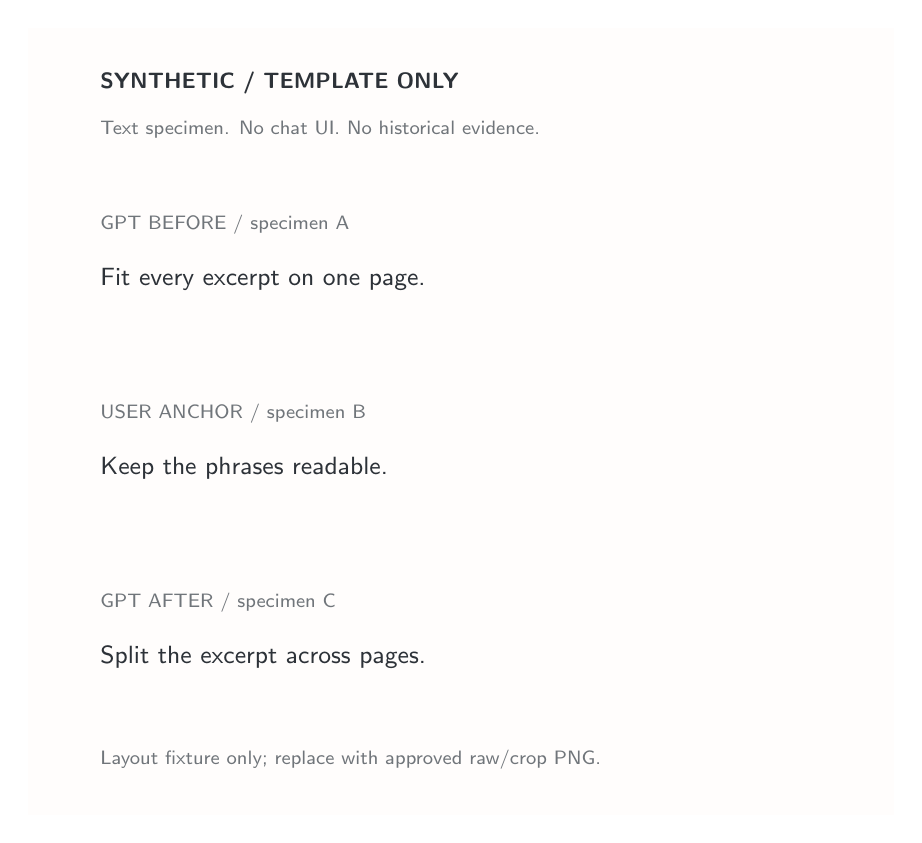
\begin{tikzpicture}[x=1mm,y=1mm]
\path[use as bounding box,fill=Panel] (0,0) rectangle (110,100);
\node[anchor=west,font=\sffamily\bfseries\footnotesize,text=Ink] at (8,93)
  {SYNTHETIC / TEMPLATE ONLY};
\node[anchor=west,font=\sffamily\scriptsize,text=Muted] at (8,87)
  {Text specimen. No chat UI. No historical evidence.};
\node[anchor=west,font=\sffamily\scriptsize,text=Muted] at (8,75) {GPT BEFORE / specimen A};
\node[anchor=west,font=\sffamily\small,text=Ink] at (8,68) {Fit every excerpt on one page.};
\node[anchor=west,font=\sffamily\scriptsize,text=Muted] at (8,51) {USER ANCHOR / specimen B};
\node[anchor=west,font=\sffamily\small,text=Ink] at (8,44) {Keep the phrases readable.};
\node[anchor=west,font=\sffamily\scriptsize,text=Muted] at (8,27) {GPT AFTER / specimen C};
\node[anchor=west,font=\sffamily\small,text=Ink] at (8,20) {Split the excerpt across pages.};
\node[anchor=west,font=\sffamily\scriptsize,text=Muted] at (8,7)
  {Layout fixture only; replace with approved raw/crop PNG.};
\end{tikzpicture}
\end{document}
